\documentclass[aspectratio=169]{beamer}

\usetheme{default}
\usecolortheme{default}
\usefonttheme{structurebold}

\setbeamertemplate{navigation symbols}{}
\setbeamertemplate{footline}[frame number]

\usepackage{amsmath}
\usepackage{booktabs}
\usepackage{multirow}
\usepackage{array}
\usepackage{tikz}
\usetikzlibrary{arrows,positioning,shapes.geometric}

\title{IO and IRIO Updating Toolkit\\and Economic Analysis}
\author{Muhammad Akmal Farouqi}
\date{2026}

\begin{document}

\begin{frame}
\titlepage
\end{frame}

\begin{frame}{Outline}
\tableofcontents
\end{frame}

%% -----------------------------------------------------------
%% PIPELINE OVERVIEW (before sections)
%% -----------------------------------------------------------

\begin{frame}{Toolkit Pipeline: Overview}
\begin{center}
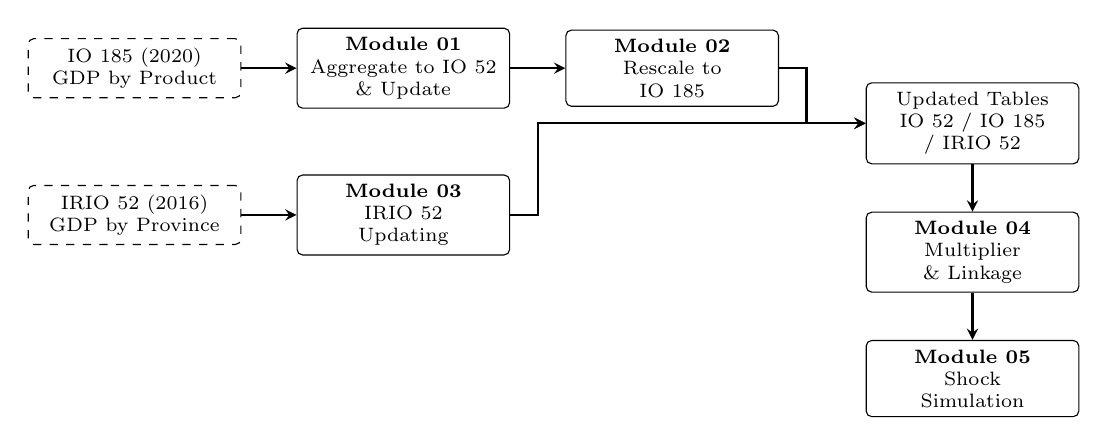
\begin{tikzpicture}[
  box/.style={rectangle, draw, rounded corners=2pt, minimum width=2.7cm,
              minimum height=0.75cm, align=center, font=\scriptsize},
  inp/.style={rectangle, draw, dashed, rounded corners=2pt, minimum width=2.7cm,
              minimum height=0.75cm, align=center, font=\scriptsize},
  arr/.style={->, >=stealth, thick},
  node distance=0.6cm and 0.7cm
]

%% --- Top branch: IO line ---
\node[inp] (d1) {IO 185 (2020)\\GDP by Product};
\node[box, right=of d1] (m01) {\textbf{Module 01}\\Aggregate to IO 52\\\& Update};
\node[box, right=of m01] (m02) {\textbf{Module 02}\\Rescale to\\IO 185};

%% --- Bottom branch: IRIO line ---
\node[inp, below=1.1cm of d1] (d2) {IRIO 52 (2016)\\GDP by Province};
\node[box, right=of d2] (m03) {\textbf{Module 03}\\IRIO 52\\Updating};

%% --- Output node, to the right of both branches, vertically centered ---
\node[box, right=1.1cm of m02, yshift=-0.7cm, minimum width=2.7cm] (out) {Updated Tables\\IO 52 / IO 185\\/ IRIO 52};

%% --- Analysis modules, below output ---
\node[box, below=0.6cm of out] (m04) {\textbf{Module 04}\\Multiplier\\\& Linkage};
\node[box, below=of m04] (m05) {\textbf{Module 05}\\Shock\\Simulation};

%% Arrows: IO line  (IO 185 -> aggregate+update IO 52 -> rescale to IO 185)
\draw[arr] (d1) -- (m01);
\draw[arr] (m01) -- (m02);

%% Arrows: IRIO line
\draw[arr] (d2) -- (m03);

%% Arrows: both branches -> output
\draw[arr] (m02.east) -- ++(0.35,0) |- (out.west);
\draw[arr] (m03.east) -- ++(0.35,0) |- (out.west);

%% Arrows: output -> analysis modules
\draw[arr] (out) -- (m04);
\draw[arr] (m04) -- (m05);

\end{tikzpicture}
\end{center}

\vspace{0.15cm}
{\footnotesize Top: IO 185 (2020) is aggregated to IO 52 and updated (M01), then rescaled back to IO 185 (M02). Bottom: IRIO 52 (2016) is updated independently (M03), in parallel with the IO line. M04 and M05 require all three updated tables.}
\end{frame}

%% -----------------------------------------------------------
\section{Input-Output Table: Overview}
%% -----------------------------------------------------------

\begin{frame}{Input-Output Table: Overview}
\tableofcontents[currentsection]
\end{frame}

\begin{frame}{Input-Output Table}
An Input-Output (IO) table is a matrix that records monetary transactions between all sectors of an economy: who buys from whom, and how much.

\medskip
\textbf{Core components:}
\begin{description}
  \item[$Z$ --- Transaction matrix] $z_{ij}$: value of goods/services sold by sector $i$ to sector $j$.
  \item[$A$ --- Technical coefficient matrix] $a_{ij} = z_{ij}/x_j$: share of input from sector $i$ required per unit of output in sector $j$.
  \item[$X$ --- Total output vector] Total production value per sector.
  \item[$Y$ --- Final demand vector] Household consumption, government, exports, investment.
\end{description}

\medskip
\textbf{Fundamental balance:}
\[
X = AX + Y \qquad \Rightarrow \qquad X = (I - A)^{-1}Y
\]
\end{frame}

%% --- NEW: IO Table Structure Illustration ---
\begin{frame}{IO Table Structure: Schematic Layout}
\begin{center}
\renewcommand{\arraystretch}{1.25}
\begin{tabular}{c|ccc|c|c}
  & \multicolumn{3}{c|}{\textbf{Intermediate Demand} ($Z$)} & \textbf{Final} & \textbf{Total} \\
  & Sector 1 & $\cdots$ & Sector $n$ & \textbf{Demand} $Y$ & \textbf{Output} $X$ \\
\hline
Sector 1       & $z_{11}$ & $\cdots$ & $z_{1n}$ & $y_1$ & $x_1$ \\
$\vdots$       & $\vdots$ & $\ddots$ & $\vdots$ & $\vdots$ & $\vdots$ \\
Sector $n$     & $z_{n1}$ & $\cdots$ & $z_{nn}$ & $y_n$ & $x_n$ \\
\hline
\textbf{Value Added} ($V$) & $v_1$ & $\cdots$ & $v_n$ & & \\
\textbf{Total Input}       & $x_1$ & $\cdots$ & $x_n$ & & \\
\end{tabular}
\end{center}

\medskip
\small
\textbf{Row balance:} $x_i = \underbrace{\sum_j z_{ij}}_{U_i \text{ (interm.\ output)}} + y_i$
\quad
\textbf{Column balance:} $x_j = \underbrace{\sum_i z_{ij}}_{V_j \text{ (interm.\ input)}} + v_j$

\medskip
The $Z$ block (intermediate transactions), $U$ (row sums of $Z$), $V$ (column sums of $Z$), $X$ (total output), and $Y$ (final demand) are the five quantities targeted by the RAS updating procedure.
\end{frame}

%% --- NEW: IO vs IRIO comparison ---
\begin{frame}{IO vs.\ IRIO: What Changes?}
\begin{columns}[T]
  \column{0.48\textwidth}
    \textbf{National IO Table}
    \begin{itemize}
      \item Dimension: $n \times n$ \\ (52 subsectors or 185 products)
      \item One block covering the entire national economy
      \item Records inter-sector transactions without spatial disaggregation
      \item Suitable for: sectoral multipliers, national policy simulation
    \end{itemize}
    \medskip
    \textit{Example code:} \texttt{I-29} = subsector 29, nationally.

  \column{0.48\textwidth}
    \textbf{Interregional IO (IRIO) Table}
    \begin{itemize}
      \item Dimension: $(n \times p) \times (n \times p)$ \\
            where $p = 34$ provinces
      \item Indonesia: $52 \times 34 = \mathbf{1{,}768}$ rows and columns
      \item Explicit inter-provincial trade flows: who in Province A buys from whom in Province B
      \item Suitable for: regional spillovers, spatial linkage, island-level analysis
    \end{itemize}
    \medskip
    \textit{Example code:} \texttt{32-I-29} = subsector I-29 in West Java (province 32).
\end{columns}

\medskip
\small
In the IRIO, the $Z$ matrix is partitioned into $p \times p$ provincial blocks:
$Z^{rs}$ = transactions \textit{from} province $r$ \textit{to} province $s$.
Diagonal blocks $Z^{rr}$ = intra-provincial; off-diagonal $Z^{rs}$ = interregional trade.
\end{frame}

%% --- EXPANDED: Why Updating ---
\begin{frame}{Why Updating is Necessary}
BPS publishes IO tables periodically, not annually. The most recent available table is the \textbf{185-product IO, base year 2020}. Up-to-date analysis for 2024 requires an updated table.

\medskip
\textbf{RAS biproportional updating} adjusts the $A$ matrix from a base year so that it is consistent with:
\begin{itemize}
  \item Target intermediate output vector $U$ (row sums of $Z$)
  \item Target intermediate input vector $V$ (column sums of $Z$)
  \item Target total output vector $X$
\end{itemize}
all derived from the most recent GDP growth data by sector.

\medskip
\textbf{IRIO requires additional attention:} the most recent IRIO published by BPS uses \textbf{base year 2016} --- an 8-year gap to 2024. Over this period, several new subsectors emerged in provinces that had no prior activity (e.g.\ coal mining in East Kalimantan, nickel in South and West Sulawesi), making direct subsector-level growth ratios undefined ($\infty$). The updating procedure must handle these structurally new subsectors explicitly.
\end{frame}

%% -----------------------------------------------------------
\section{RAS Method}
%% -----------------------------------------------------------

\begin{frame}{RAS Method}
\tableofcontents[currentsection]
\end{frame}

\begin{frame}{RAS: Principle}
RAS is a biproportional iterative procedure that scales an initial $A$ matrix (seed) until its implied row and column sums match target vectors.

\medskip
Each iteration consists of two steps:
\begin{enumerate}
  \item \textbf{Row scaling (R):} scale each row so that $\text{rowSums}(A \cdot X) = U_{\text{target}}$
  \item \textbf{Column scaling (S):} scale each column so that $\text{colSums}(A \cdot X) = V_{\text{target}}$
\end{enumerate}
Iteration continues until $\max(\text{row error}, \text{col error}) < \varepsilon$.

\medskip
\textbf{Target vectors} are derived from base-year values scaled by GDP growth rates:
\[
U_j^{2024} = U_j^{2020} \cdot g_j, \quad
V_j^{2024} = V_j^{2020} \cdot g_j, \quad
X_j^{2024} = X_j^{2020} \cdot g_j
\]
where $g_j$ is the GDP growth ratio of sector $j$ from base year to 2024.
\end{frame}

\begin{frame}{RAS: Convergence Requirements}
\begin{enumerate}
  \item \textbf{Balance constraint (mandatory):}
  \[
  \sum U_{\text{target}} = \sum V_{\text{target}}
  \]
  $V$ is rescaled to match $\sum U$ before iteration begins. Without this, RAS will not converge.

  \item \textbf{Non-zero seed for new sectors:}\\
  Sectors with a positive target but an all-zero column in the base-year $A$ cannot be updated from structural zeros. A non-zero seed is required (method differs between IO and IRIO --- see respective modules).

  \item \textbf{Positive index:}\\
  Only sectors where $X > 0$, $U > 0$, and $V > 0$ are included in the iteration. Sectors outside this index remain at zero and do not participate in scaling.
\end{enumerate}
\end{frame}

%% -----------------------------------------------------------
\section{Module 1 --- IO 52-Subsector Updating}
%% -----------------------------------------------------------

\begin{frame}{Module 1 --- IO 52-Subsector Updating}
\tableofcontents[currentsection]
\end{frame}

%% --- NEW: Data Requirements ---
\begin{frame}{Module 1: Data Requirements}
\begin{center}
\renewcommand{\arraystretch}{1.3}
\scriptsize
\begin{tabular}{@{}p{5.0cm}p{1.0cm}p{6.6cm}@{}}
\toprule
\textbf{File} & \textbf{Format} & \textbf{Content} \\
\midrule
\texttt{io20.csv} & CSV & IO 185 (2020), product-level format (base table) \\
\texttt{io16(52).csv} & CSV & IO 52 (2016), subsector-level format (I-46 reference) \\
\texttt{regional\_gdp\_52\_subsectors.xlsx} & xlsx & GDP per subsector, growth rates 2020--2024 \\
\texttt{concordance\_185\_52\_17.xlsx} & xlsx & Mapping: 185 products $\to$ 52 subsectors $\to$ 17 sectors \\
\bottomrule
\end{tabular}
\end{center}

\medskip
\small
The concordance table is the key structural input: it defines which of the 185 product rows and columns aggregate to each of the 52 subsectors. IO 52 (2016) is used exclusively for reconstructing subsector I-46.
\end{frame}

\begin{frame}{Module 1: IO 52-Subsector Updating (2020 $\to$ 2024)}
\textbf{Objective:} produce a 52-subsector IO table for 2024 from the 185-product IO table of 2020.

\medskip
\textbf{Workflow:}
\begin{enumerate}
  \item \textbf{Aggregation} --- collapse IO 185-product to 52-subsector using a concordance table (sum rows and columns by mapping).
  \item \textbf{Reconstruction of subsector I-46} --- I-46 (Other Financial Services) is absent from the 2020 IO in 52-subsector format. It is estimated from the I-46 share within (I-43+I-44+I-45+I-46) in the 2016 IO table.
  \item \textbf{Target vector preparation} --- compute $U$, $V$, $X$ for 2024 using GDP growth rates per subsector; rescale $V$ so $\sum V = \sum U$.
  \item \textbf{RAS iteration} --- run until row and column errors $< 10^{-20}$.
\end{enumerate}

\medskip
\textbf{Output:} \texttt{io\_2024(52x52).xlsx} --- sheets: $A$, $Z$, $U$, $V$, $X$, consistency evaluation.
\end{frame}

%% --- NEW: Why I-46 is absent ---
\begin{frame}{Why Subsector I-46 is Absent from IO 2020}
IO 2020 from BPS is published in \textbf{185-product format}. To use it in a 52-subsector framework, rows and columns must be aggregated via a concordance table.

\medskip
Subsector \textbf{I-46 (Other Financial Services / Jasa Penunjang Keuangan)} has \textit{no product code} in the 185-product classification --- meaning there is no row or column in IO 2020 that maps to I-46. It therefore cannot appear after aggregation.

\medskip
\textbf{Why does IO 2016 have I-46?} IO 2016 is published directly in the 52-subsector format by BPS, where I-46 already exists as a standalone entry.

\medskip
\textbf{Solution:} use the 2016 IO as a structural reference. The \textit{share} of I-46 within the group (I-43+I-44+I-45+I-46) is computed from 2016 and applied to the 2020 values of (I-43+I-44+I-45) to recover an I-46 estimate. The group total is preserved after redistribution.
\end{frame}

\begin{frame}{Reconstruction of Subsector I-46}
\textbf{Procedure:}
\begin{enumerate}
  \item Compute I-46 column share from 2016: for each column $j$,
  \[
  \phi_j^{\text{col}} = \frac{z_{46,j}^{2016}}{z_{43,j}^{2016}+z_{44,j}^{2016}+z_{45,j}^{2016}+z_{46,j}^{2016}}
  \]
  and analogously row shares $\phi_i^{\text{row}}$.
  \item Apply shares to 2020 values of (I-43+I-44+I-45):
  \[
  \hat{z}_{46,j}^{2020} = \phi_j^{\text{col}} \cdot \bigl(z_{43,j}^{2020}+z_{44,j}^{2020}+z_{45,j}^{2020}\bigr)
  \]
  \item Reduce I-43, I-44, I-45 proportionally so the \textbf{group total is preserved}:
  \[
  z_{k,j}^{\text{adj}} = z_{k,j}^{2020} - \frac{z_{k,j}^{2020}}{z_{43,j}^{2020}+z_{44,j}^{2020}+z_{45,j}^{2020}} \cdot \hat{z}_{46,j}^{2020}, \quad k \in \{43,44,45\}
  \]
\end{enumerate}
\end{frame}

%% --- NEW: Module 1 Evaluation Results ---
\begin{frame}{Module 1: RAS Evaluation Results}
\textbf{Convergence tolerance:} $\varepsilon = 10^{-20}$ (machine precision target)

\medskip
\begin{center}
\renewcommand{\arraystretch}{1.3}
\footnotesize
\begin{tabular}{@{}p{5.2cm}rrl@{}}
\toprule
\textbf{Metric} & \textbf{Value (Rp)} & \textbf{Relative (\%)} & \textbf{Assessment} \\
\midrule
Row consistency $\max|AX - U|$              & 2.50e$-$01    & $5.03 \times 10^{-16}$\% & \textit{machine zero} \\
Column consistency $\max|\text{col}(AX)-V|$ & 0.00e$+$00    & 0.00\%                   & \textit{exact} \\
\midrule
Total output $X$            & 4.97e$+$16 Rp & --- & --- \\
Total intermediate flow $Z$ & 2.04e$+$16 Rp & --- & --- \\
\bottomrule
\end{tabular}
\end{center}

\medskip
\small
Relative values computed as error divided by total output $X = \text{Rp}\;4.97 \times 10^{16}$. Both row and column residuals are far below the 5\% materiality threshold --- the updated IO 52 (subsector) matrix is internally consistent at machine precision. No seeded subsectors were required (all 52 subsectors had non-zero structure in IO 185 (2020)).
\end{frame}

%% -----------------------------------------------------------
\section{Module 2 --- Rescaling to IO 185 Products}
%% -----------------------------------------------------------

\begin{frame}{Module 2 --- Rescaling to IO 185 Products}
\tableofcontents[currentsection]
\end{frame}

%% --- NEW: Data Requirements ---
\begin{frame}{Module 2: Data Requirements}
\begin{center}
\renewcommand{\arraystretch}{1.3}
\scriptsize
\begin{tabular}{@{}p{5.0cm}p{1.0cm}p{6.6cm}@{}}
\toprule
\textbf{File} & \textbf{Format} & \textbf{Content} \\
\midrule
\texttt{io\_2024(52x52).xlsx} & xlsx & Module 01 output: $A$, $Z$, $X$ in subsector (IO 52) format \\
\texttt{io20.csv} & CSV & IO 185 (2020), product-level format (disaggregation weights) \\
\texttt{concordance\_185\_52\_17.xlsx} & xlsx & Mapping: 185 products $\leftrightarrow$ 52 subsectors \\
\bottomrule
\end{tabular}
\end{center}

\medskip
\small
IO 185 (2020) serves as the \textit{proportion reference}: the within-subsector product structure is assumed unchanged from 2020 to 2024. The 2024 subsector totals (from Module 01) are then split across individual products using these 2020 proportions.
\end{frame}

\begin{frame}{Module 2: Rescaling IO 52 $\to$ IO 185 Products (2024)}
\textbf{Objective:} disaggregate the 52-subsector result from Module 1 into a full 185-product IO table for 2024.

\medskip
\textbf{I-46 reversal (pre-processing):} before disaggregation, I-46 is redistributed back into I-43/44/45 proportionally --- the 185-product IO has no I-46 product code.

\medskip
\textbf{Disaggregation formula:} for each subsector pair $(K, L)$, individual product cell $(k, l)$:
\[
Z_{kl}^{2024} = Z_{KL}^{2024} \cdot \frac{Z_{kl}^{2020}}{Z_{KL}^{2020}}
\]
Within-subsector structure is assumed unchanged from 2020 to 2024.

\medskip
\textbf{Special case:} if $Z_{KL}^{2020} = 0$ but $Z_{KL}^{2024} > 0$ (new transaction link in 2024), the 2024 value is distributed \textit{equally} across all $(k,l)$ cells in that block.

\medskip
\textbf{Output:} \texttt{io\_2024(185x185).xlsx} --- sheets: $A$, $Z$, $U$, $V$, $X$, eval summary, eval diagonal.
\end{frame}

\begin{frame}{Consistency Verification}
After disaggregation, $Z_{185}^{2024}$ is re-aggregated back to the 51-subsector level and compared against $Z_{51}^{2024}$ from Module 1.

\medskip
\textbf{Metrics checked:}
\begin{itemize}
  \item Maximum absolute difference across all cells: must approach 0
  \item Relative maximum difference: must approach 0
  \item Total sum of $Z_{185}$ vs total sum of $Z_{51}$: must be equal
  \item Diagonal entries per subsector (intra-subsector transactions): top-10 deviations reported
\end{itemize}
\end{frame}

%% --- NEW: Module 2 Evaluation Results ---
\begin{frame}{Module 2: Disaggregation Evaluation Results}
\textbf{Test:} re-aggregate $Z_{185}^{2024}$ back to 51 subsectors, compare to $Z_{51}^{2024}$ from Module 01.

\medskip
\begin{center}
\renewcommand{\arraystretch}{1.3}
\begin{tabular}{lrrl}
\toprule
\textbf{Metric} & \textbf{Value (Rp)} & \textbf{Relative (\%)} & \textbf{Assessment} \\
\midrule
Max absolute diff (any cell) & 6.25e$-$02 & $3.07 \times 10^{-16}$\% & \textit{machine zero} \\
Relative max difference      & 8.997e$-$17 & $8.997\times10^{-15}$\% & \textit{machine zero} \\
Total $Z_{185}$ sum          & 2.0382e$+$16 Rp & --- & --- \\
Total $Z_{51}$ sum           & 2.0382e$+$16 Rp & --- & --- \\
Sum difference               & 0.00e$+$00 & 0.00\% & \textit{exact} \\
\bottomrule
\end{tabular}
\end{center}

\medskip
\small
The largest per-cell discrepancy is Rp 0.0625 on a total flow of Rp $2.04 \times 10^{16}$ --- a relative error of order $10^{-16}$\%, well within machine precision. The subsector with the largest diagonal deviation is \textbf{I-44} at Rp 2.44e$-$04, which is $1.44 \times 10^{-14}$\% of its own flow value. Disaggregation is exact within floating-point arithmetic.
\end{frame}

%% -----------------------------------------------------------
\section{Module 3 --- IRIO 52-Subsector Updating}
%% -----------------------------------------------------------

\begin{frame}{Module 3 --- IRIO 52-Subsector Updating}
\tableofcontents[currentsection]
\end{frame}

\begin{frame}{Interregional Input-Output (IRIO)}
The IRIO table extends the national IO by adding a \textbf{spatial dimension}: each province is treated as a separate economic block, with explicit interregional trade flows.

\medskip
\textbf{Format for Indonesia:}
\begin{itemize}
  \item 34 provinces $\times$ 52 subsectors = \textbf{1,768 rows and columns}
  \item Matrix dimension: $1768 \times 1768$
  \item Captures both intra-provincial and inter-provincial transactions
\end{itemize}

\medskip
\textbf{Additional analytical questions enabled by IRIO:}
\begin{itemize}
  \item How does an investment shock in Province A affect output in Province B?
  \item Which provinces are most structurally integrated into national supply chains?
  \item How do interregional linkages differ across islands?
\end{itemize}
\end{frame}

%% --- NEW: Data Requirements ---
\begin{frame}{Module 3: Data Requirements}
\begin{center}
\renewcommand{\arraystretch}{1.3}
\scriptsize
\begin{tabular}{@{}p{5.0cm}p{1.0cm}p{6.6cm}@{}}
\toprule
\textbf{File} & \textbf{Format} & \textbf{Content} \\
\midrule
\texttt{irio16.csv} & CSV & IRIO 52 (2016), subsector $\times$ 34 provinces (base table) \\
\texttt{regional\_gdp\_52\_subsectors.xlsx} & xlsx & GDP per subsector per province, 2016 and 2024 \\
\texttt{concordance\_185\_52\_17.xlsx} & xlsx & Mapping: 52 subsectors $\to$ 17 sectors \\
\bottomrule
\end{tabular}
\end{center}

\medskip
\small
The IRIO 52 (2016) matrix has dimension $1768 \times 1768$ ($52 \times 34$ province-subsector pairs). Subsector codes follow the format \texttt{provcode-subsectorcode} (e.g.\ \texttt{32-I-29}). The GDP file must include both base-year (2016) and target-year (2024) values per province-subsector combination.
\end{frame}

%% --- NEW: Why aggregate to 17 first ---
\begin{frame}{Why Aggregate to 17 Sectors First?}
Direct subsector-level growth ratios $g_s = \text{GDP}_{s,p}^{2024} / \text{GDP}_{s,p}^{2016}$ are \textbf{undefined} ($\infty$) when a subsector had zero output in 2016 but positive output in 2024. This occurs for subsectors that \textit{emerged after 2016} in specific provinces.

\medskip
\textbf{Examples of structurally new province-subsector pairs:}

\begin{center}
\renewcommand{\arraystretch}{1.2}
\begin{tabular}{clcrr}
\toprule
\textbf{Prov.} & \textbf{Province} & \textbf{Subsector} & \textbf{Base 2016 (Rp M)} & \textbf{Target 2024 (Rp M)} \\
\midrule
64 & Kalimantan Timur  & I-22 & 0 & 894.07 \\
76 & Sulawesi Barat    & I-09 & 0 &  57.99 \\
13 & Sumatera Barat    & I-14 & 0 &  18.38 \\
73 & Sulawesi Selatan  & I-09 & 0 &   2.64 \\
\bottomrule
\end{tabular}
\end{center}

\medskip
\small
Directly applying $g_s = \infty$ into RAS causes NaN propagation and divergence. The 2-step aggregation resolves this: the \textbf{parent sector} (17-sector level) almost always has a finite, economically meaningful growth rate even when some of its subsectors are new.
\end{frame}

\begin{frame}{Module 3: IRIO 52-Subsector Updating (2016 $\to$ 2024)}
\textbf{Workflow:}
\begin{enumerate}
  \item \textbf{Aggregate IRIO 52 $\to$ 17 sectors} per province. Update $U$, $V$, $X$ at the 17-sector level using provincial GDP growth rates $g_S = X_S^{2024}/X_S^{2016}$.
  \item \textbf{Disaggregate back to 52 subsectors} using target-year GDP proportions:
  \[
  X_{s,p}^{2024} = \frac{\text{GDP}_{s,p}^{2024}}{\text{GDP}_{S,p}^{2024}} \cdot X_{S,p}^{2024,\text{updated}}
  \]
  where $s$ = subsector, $S$ = parent 17-sector, $p$ = province. The share $\text{GDP}_{s,p}^{2024}/\text{GDP}_{S,p}^{2024}$ is always well-defined and bounded in $[0,1]$.
  \item \textbf{RAS} on the $1768 \times 1768$ matrix until convergence.
\end{enumerate}

\medskip
By anchoring growth at the 17-sector level, all growth ratios remain finite. Subsector-level variation is recovered in step 2 through the 2024 GDP composition.
\end{frame}

\begin{frame}{Seed Strategy for New Subsectors in IRIO}
Subsectors absent in 2016 (total input $= 0$) but with positive 2024 targets have an all-zero $A$ column --- RAS cannot scale from zero.

\medskip
\textbf{Island-based donor approach:}
\begin{enumerate}
  \item Identify provinces on the \textbf{same island} that have the same subsector active in 2016.
  \item Use the column/row mean of those donor provinces as the seed $A$ column/row.
  \item If no donors exist on the same island: fall back to the \textbf{national mean} across all provinces with that subsector active.
\end{enumerate}

\medskip
\textbf{Island mapping (province code):} Sumatera $(<30)$, Jawa $(<40)$, Bali-Nusra $(<60)$, Kalimantan $(<70)$, Sulawesi $(<80)$, Maluku $(<90)$, Papua $(\geq 90)$.

\medskip
\textbf{Rationale:} island-based donors are preferred over national average because production structures are more geographically homogeneous within an island than across the full archipelago.
\end{frame}

%% --- NEW: Module 3 Evaluation Results ---
\begin{frame}{Module 3: IRIO RAS Evaluation Results}
\textbf{Matrix size:} $1768 \times 1768$ ($52$ subsectors $\times$ 34 provinces). \textbf{Tolerance:} $\varepsilon = 10^{-10}$.

\medskip
\begin{center}
\renewcommand{\arraystretch}{1.3}
\footnotesize
\begin{tabular}{@{}p{5.2cm}rrl@{}}
\toprule
\textbf{Metric} & \textbf{Value (Rp)} & \textbf{Relative (\%)} & \textbf{Assessment} \\
\midrule
Row consistency $\max|AX - U|$              & 6.42e$+$13    & 0.154\%                & \textit{within 5\% threshold} \\
Column consistency $\max|\text{col}(AX)-V|$ & 6.25e$-$02    & $1.50\times10^{-16}$\% & \textit{machine zero} \\
Total output $X$                            & 4.17e$+$16 Rp & ---                    & --- \\
\bottomrule
\end{tabular}
\end{center}

\medskip
\small
\textbf{Interpretation:} Column consistency is at machine precision. The row residual of Rp $6.42 \times 10^{13}$ is large in absolute terms but represents only \textbf{0.154\%} of total output --- well within the 5\% materiality threshold. This residual reflects floating-point accumulation across the $1768 \times 1768$ system and is structurally expected for a matrix of this dimension. The IRIO 52 table is internally consistent for applied analysis.
\end{frame}

%% -----------------------------------------------------------
\section{Module 4 --- Multiplier and Linkage Analysis}
%% -----------------------------------------------------------

\begin{frame}{Module 4 --- Multiplier and Linkage Analysis}
\tableofcontents[currentsection]
\end{frame}

%% --- NEW: Data Requirements ---
\begin{frame}{Module 4: Data Requirements}
\begin{center}
\renewcommand{\arraystretch}{1.2}
\footnotesize
\begin{tabular}{@{}p{4.2cm}p{3.0cm}p{4.2cm}@{}}
\toprule
\textbf{File} & \textbf{Sheet} & \textbf{Content} \\
\midrule
\texttt{io\_2024(52x52).xlsx} & \texttt{a\_io52\_2024} & $A$ matrix, 52 subsectors \\
 & \texttt{totaloutput\_2024} & $X$ vector \\
 & \texttt{interm\_output\_2024} & $U$ vector (for $Y = X - U$) \\
\texttt{io\_2024(185x185).xlsx} & \texttt{a\_io185\_2024} & $A$ matrix, 185 products \\
\texttt{irio\_2024(1768x1768).xlsx} & \texttt{a\_irio\_2024} & $A$ matrix, 1768 province-subsectors \\
\bottomrule
\end{tabular}
\end{center}

\medskip
\small
The final demand vector $Y = X - U$ is derived internally. All three tables are processed independently; outputs are exported to separate xlsx files under the \texttt{03 Output} folder, subfolder \texttt{Multiplier results}.
\end{frame}

\begin{frame}{Leontief Multiplier (Demand Side)}
\textbf{Leontief inverse:} $L = (I - A)^{-1}$

$L_{ij}$ captures the total output required from sector $i$ per unit of final demand injected into sector $j$, including all direct and indirect rounds of production.

\medskip
\textbf{Derived indicators:}
\begin{description}
  \item[Output Multiplier (OM)] $OM_j = \sum_i L_{ij}$ (column sum of $L$). Total economy-wide output induced per unit of final demand in sector $j$.
  \item[Backward Linkage (BL)] Hirschman-Rasmussen normalized OM:
  \[
  BL_j = \frac{OM_j / n}{\sum_{i,j} L_{ij} / n^2}
  \]
  $BL > 1$: sector $j$ pulls above-average input demand from the rest of the economy.
\end{description}
\end{frame}

\begin{frame}{Ghosh Multiplier (Supply Side)}
\textbf{Output coefficient matrix:} $B_{ij} = z_{ij}/x_i$ --- share of sector $i$'s output flowing to sector $j$.

\textbf{Ghosh inverse:} $G = (I - B)^{-1}$

$G_{ij}$ captures total output generated in sector $j$ per unit of primary input added to sector $i$.

\medskip
\textbf{Derived indicators:}
\begin{description}
  \item[Supply Multiplier (SM)] $SM_i = \sum_j G_{ij}$ (row sum of $G$). Total downstream output induced per unit of primary input in sector $i$.
  \item[Forward Linkage (FL)] Hirschman-Rasmussen normalized SM:
  \[
  FL_i = \frac{SM_i / n}{\sum_{i,j} G_{ij} / n^2}
  \]
  $FL > 1$: sector $i$ supplies above-average inputs to downstream sectors.
\end{description}

\medskip
\small Note: Ghosh is used here for FL measurement only. Causal supply-side simulation uses HEM (Oosterhaven, 1988).
\end{frame}

\begin{frame}{Hypothetical Extraction Method (HEM)}
HEM measures total output loss if a sector is fully removed from the economy, capturing backward and forward effects simultaneously without double-counting.

\medskip
\textbf{Procedure for each sector $k$:}
\begin{enumerate}
  \item Baseline: $X^* = L \cdot Y$
  \item Zero out row $k$ and column $k$ in $A$ $\to$ $A^{\text{ext}}$
  \item $L^{\text{ext}} = (I - A^{\text{ext}})^{-1}$; $\quad X^{\text{ext}} = L^{\text{ext}} \cdot Y$
  \item $TL_k = \sum X^* - \sum X^{\text{ext}}$
\end{enumerate}

\medskip
\textbf{Decomposition:}
\begin{itemize}
  \item $BL_{\text{HEM},k}$: output loss when only column $k$ is zeroed (sector stops purchasing)
  \item $FL_{\text{HEM},k}$: output loss when only row $k$ is zeroed (sector stops supplying)
  \item $TL_{\text{HEM},k}$: full extraction loss; the definitive structural importance measure
  \item $nTL_k = TL_k / \overline{TL}$: $>1$ indicates above-average structural importance
\end{itemize}
\end{frame}

\begin{frame}{Sector Classification and Indicator Summary}
\textbf{Hirschman-Rasmussen classification:}

\medskip
\begin{center}
\begin{tabular}{ccc}
\toprule
\textbf{BL} & \textbf{FL} & \textbf{Sector type} \\
\midrule
$>1$ & $>1$ & Key sector \\
$>1$ & $\leq 1$ & Backward-dependent \\
$\leq 1$ & $>1$ & Forward-dependent \\
$\leq 1$ & $\leq 1$ & Independent \\
\bottomrule
\end{tabular}
\end{center}

\medskip
$nTL > 1$ (HEM criterion) identifies structurally important sectors independently of the HR classification.

\medskip
All indicators are computed for IO 52, IO 185, and IRIO 52. For IRIO, results are additionally aggregated by province and by national subsector average.
\end{frame}

%% --- NEW: How to Read Multiplier Output ---
\begin{frame}{How to Read Multiplier Output}
\textbf{Sheet \texttt{linkage}} (one row per sector): columns BL, FL, OM, SM, nTL, and HR classification.

\medskip
\textbf{Example interpretation (IO 52):}
\begin{itemize}
  \item Sector \textbf{I-28} has the highest $OM = 2.790$: every Rp\,1\,T of additional final demand in I-28 induces \textbf{Rp\,2.79\,T} of total economy-wide output.
  \item Sector \textbf{I-31} has the highest $nTL = 5.439$: if I-31 is extracted from the economy, output loss is \textbf{5.4$\times$ the average} sector extraction loss.
\end{itemize}

\medskip
\textbf{HR vs.\ HEM:}
\begin{itemize}
  \item HR (BL/FL) uses the Leontief/Ghosh inverse --- a linear approximation. It can underestimate importance for large sectors where non-linearities matter.
  \item HEM computes the full counterfactual (non-linear). It is the preferred criterion for identifying structurally critical sectors.
\end{itemize}

\medskip
\textbf{IRIO additional sheets:} \texttt{linkage\_prov} aggregates BL/FL/nTL per province (34 rows); \texttt{linkage\_nat} aggregates per subsector across all 34 provinces (52 rows).
\end{frame}

%% --- NEW: Summary Statistics ---
\begin{frame}{Module 4: Summary Statistics}
\begin{center}
\renewcommand{\arraystretch}{1.05}
\footnotesize
\begin{tabular}{@{}lrrr@{}}
\toprule
\textbf{Indicator} & \textbf{IO 52 (subsector)} & \textbf{IO 185 (product)} & \textbf{IRIO 52 (prov.-subsector)} \\
\midrule
Total units                    & 52           & 185          & 1{,}768 \\
Key (BL$>$1, FL$>$1)            & 12           & 42           & 197 \\
Backward-dependent              & 15           & 65           & 239 \\
Forward-dependent               & 13           & 47           & 649 \\
Independent                     & 12           & 31           & 683 \\
HEM important ($nTL > 1$)       & 17           & 44           & 246 \\
\midrule
OM range                        & [1.21, 2.79] & [1.04, 2.80] & [1.00, 3.81] \\
BL range                        & [0.74, 1.71] & [0.64, 1.72] & [0.88, 3.35] \\
FL range                        & [0.57, 1.75] & [0.55, 1.96] & [0.57, 3.07] \\
$nTL$ range                     & [0.06, 5.44] & [0.00, 14.58] & [0.00, 72.55] \\
\midrule
Top by OM                       & I-28 (2.79)  & 145 (2.80)   & 82-I-28 (3.81) \\
Top by $nTL$                    & I-31 (5.44)  & 156 (14.58)  & 31-I-31 (72.55) \\
\midrule
Top province by $\overline{nTL}$ & ---         & ---          & Prov.\ 32 (6.12) \\
\bottomrule
\end{tabular}
\end{center}

\medskip
\small
``Top by OM/$nTL$'' for IO 185 reports the product code; for IRIO 52 it reports province-subsector code (province code -- subsector code).
\end{frame}

%% -----------------------------------------------------------
\section{Module 5 --- Shock Simulation}
%% -----------------------------------------------------------

\begin{frame}{Module 5 --- Shock Simulation}
\tableofcontents[currentsection]
\end{frame}

%% --- NEW: Data Requirements ---
\begin{frame}{Module 5: Data Requirements}
\begin{center}
\renewcommand{\arraystretch}{1.2}
\begin{tabular}{lll}
\toprule
\textbf{File} & \textbf{Sheet} & \textbf{Content} \\
\midrule
\texttt{io\_2024(52x52).xlsx}       & $A$, $X$, $U$, $V$ & IO 52 matrices and vectors \\
\texttt{io\_2024(185x185).xlsx}     & $A$, $X$, $U$, $V$ & IO 185 matrices and vectors \\
\texttt{irio\_2024(1768x1768).xlsx} & $A$, $X$, $U$, $V$ & IRIO matrices and vectors \\
\bottomrule
\end{tabular}
\end{center}

\medskip
Leontief ($L$) and Ghosh ($G$) inverses are re-computed within this script. The final demand vector $Y = X - U$ and primary input vector $V$ are derived internally. Scenarios are defined directly in the \texttt{scenarios} list at the top of the script.
\end{frame}

\begin{frame}{Module 5: Demand and Supply Shock Simulation}
\textbf{Objective:} batch simulation of economy-wide output impacts from user-defined shocks.

\medskip
\textbf{Demand shock (Leontief):} final demand increases by $\Delta Y$ in sector $j$:
\[
\Delta X = L \cdot \Delta Y
\]
$\Delta X_i$ = output increase induced in sector $i$ from the demand injection. Captures backward (upstream) propagation.

\medskip
\textbf{Supply shock (Ghosh):} primary input supply increases by $\Delta V$ in sector $i$:
\[
\Delta X = \Delta V \cdot G
\]
$\Delta X_j$ = output increase induced in sector $j$ from the supply expansion. Captures forward (downstream) propagation.

\medskip
Shocks are defined in a \texttt{scenarios} list and executed in batch via \texttt{run\_batch()}.
\end{frame}

\begin{frame}{IRIO Shock Modes}
For IRIO, shocks can be applied in three modes:

\medskip
\begin{description}
  \item[Direct] Shock at a single province-subsector pair.\\
        Example: \texttt{32-I-29} targets subsector I-29 in West Java (province 32).

  \item[Subsector national] Shock distributed across all 34 provinces for one subsector, proportional to each province's output share in that subsector.\\
        Example: a national demand increase for subsector I-01 (Agriculture).

  \item[Province all] Shock distributed across all 52 subsectors within one province, proportional to each subsector's output share.\\
        Example: a provincial stimulus package for all subsectors in Papua (province 94).
\end{description}

\medskip
For IO 52 and IO 185, the mode is always direct.
\end{frame}

%% --- NEW: How Shock Propagation Works ---
\begin{frame}{How Shock Propagation Works}
\textbf{Demand shock (backward propagation):}

A demand injection $\Delta Y_j$ into sector $j$ triggers upstream production: sector $j$ needs more inputs $\to$ its suppliers increase output $\to$ their suppliers increase output, and so on. The full chain is captured by:
\[
\Delta X_i = L_{ij} \cdot \Delta Y_j \quad \text{(output increase in sector } i \text{)}
\]

\medskip
\textbf{Supply shock (forward propagation):}

A primary input expansion $\Delta V_i$ in sector $i$ enables sector $i$ to produce more $\to$ downstream users receive more inputs $\to$ they can expand output further:
\[
\Delta X_j = \Delta V_i \cdot G_{ij} \quad \text{(output increase in sector } j \text{)}
\]

\medskip
\textbf{Output columns in result sheet:} \texttt{delta\_output} (absolute, Rp), \texttt{pct\_of\_baseline} (impact as \% of sector baseline $X$), and effective multiplier $= \sum \Delta X / \text{shock value}$ in \texttt{batch\_summary}.

\medskip
\small \textbf{Caveat:} Ghosh supply simulation is an accounting framework, not a causal model. Treat supply shock results as directional indicators, not structural predictions (Oosterhaven, 1988).
\end{frame}

\begin{frame}{Reading Simulation Output}
\textbf{Output:} \texttt{shock\_simulation.xlsx} --- one sheet per scenario plus a \texttt{batch\_summary} sheet.

\medskip
\textbf{Columns per scenario sheet:}

\medskip
\begin{center}
\begin{tabular}{ll}
\toprule
\textbf{Column} & \textbf{Content} \\
\midrule
\texttt{kode}            & Subsector/product code (or province-subsector for IRIO) \\
\texttt{delta\_input}    & Shock magnitude applied (Rp trillion) \\
\texttt{delta\_output}   & Output impact in that subsector/product \\
\texttt{X\_baseline}     & Total output in 2024 (pre-shock) \\
\texttt{pct\_of\_baseline} & Impact as \% of baseline output \\
\bottomrule
\end{tabular}
\end{center}

\medskip
\texttt{batch\_summary} reports total impact, effective multiplier ($= \Delta X_{\text{total}} / \text{shock value}$), and the most-affected sector for every scenario.
\end{frame}

%% -----------------------------------------------------------

\begin{frame}{}
\begin{center}
\Large Thank you.
\end{center}
\end{frame}

\end{document}